\documentclass[12pt, onecolumn]{article}


\usepackage[utf8]{inputenc}
\usepackage[italian]{babel}

\usepackage{graphicx}
\usepackage{enumitem}

%opening
\title{Time Series Final Project}
\author{Pranav Kasela \\$846965$}
\date{}
\begin{document}

\maketitle

\section*{Introduction}
Lo scopo del progetto è studiare una serie temporale riguardante dati dell'elettricità, facendo una previsione sul suo andamento nell'anno successivo (2019), per cui verranno utilizzate tre metodologie diverse: ARIMA, UCM e reti neurali ricorsive.\\
Per confrontare tale metodologie verrà utilizzata la metrica MAPE e confronto visivo, poiché un modello potrebbe fare una predizione costante e ottenere un MAPE comunque basso.
\begin{figure}[!h]
  \centering
  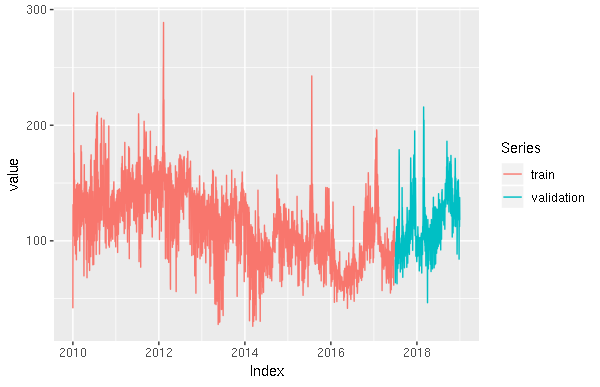
\includegraphics[width=\linewidth, height=7cm]{imgs/Series.png}
  \caption{Grafico della Serie}
  \label{fig:series}
\end{figure}\\
Dal dataset l'ultimo anno e mezzo viene tenuto separato (Figura \ref{fig:series}), esso fungerà da validation set sul quale verranno confrontati le varie metodologie di previsione.
Come metrica è stata scelta MAPE perché più facile da capire da un punto di vista umano, si poteva benissimo scegliere anche la MSE o la MAE.
Mentre per il confronto nelle metodologie stesse, i.e., modelli con diversi iper-parametri o architetture si sceglieranno delle metriche diverse, e verranno dette quando si spiega ciascun modello.
%test è quello che verrà usato alla fine dai prof....
\section*{ARIMA}
Si usa la classe xts per definire la serie temporale (xts perché la serie è giornaliera nei vari anni), plottando ACF e PACF (Figura \ref{fig:ACF_1}) si vede immediatamente l'esistenza di tutte tre componenti stagionali con stagionalità 7: AR$(1)_7$I$(1)_7$MA$(1)_7$ poiché si vede una discesa geometrica (ogni 7 giorni) nel grafico della PACF e una discesa lineare (ogni 8 giorni) nel grafico della ACF, l'esistenza della parte di integrazione stagionale si può vedere anche facendo un modello SARMA$(1,1)_7$ e vedendo che il coefficiente di SAR risulta essere molto vicino ad 1. 
\begin{figure}[!h]
  \centering
  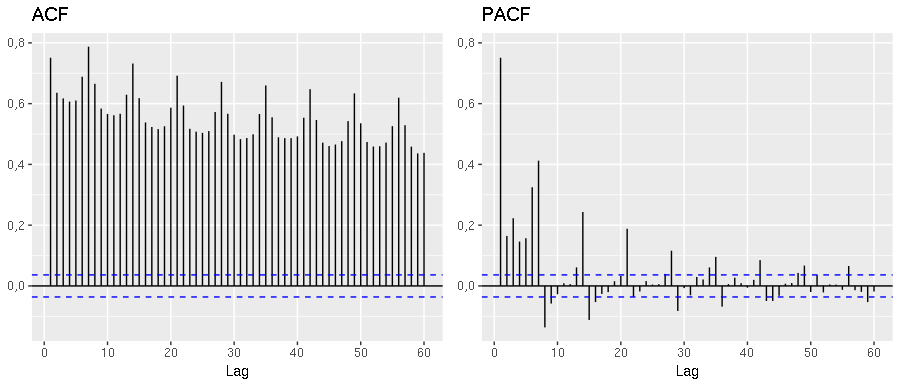
\includegraphics[width=\linewidth,height=5cm]{imgs/ACF_1.png}
  \caption{ACF e PACF della Serie.}
  \label{fig:ACF_1}
\end{figure}\\
Vi sembra essere anche quale componente non stagionale oltre ad una possibile parte di integrazione dovuta all'esistenza di qualche trend nella serie, ciò viene studiato sui residui dopo aver applicato il modello SARIMA$(1,1,1)_7$.
Sui grafici della ACF/PACF dei residui (Figura \ref{fig:ACF_2}) si vede che c'è un modello ARMA ma non si riesce a capire facilmente quali siano i coefficienti.
Per questa ragione si effettua una Grid Search con i coefficienti (potenze del polinomio caratteristico) di AR e MA che variano da 0 a 6, e scegliamo il modello con la log-likelihood più alta: Il modello con la log-likelihood più alta risulta essere un ARMA(6,6), calcolando i moduli delle radici si vede che sono molto vicini ad 1, ciò significa che la serie aveva, come già si sospettava,  una parte di integrazione, si prova con la prima integrazione e questo problema viene risolto, quindi il modello finale proposto è un ARIMA$(6,1,6)(1,1,1)_7$.\\
\begin{figure}[!h]
  \centering
  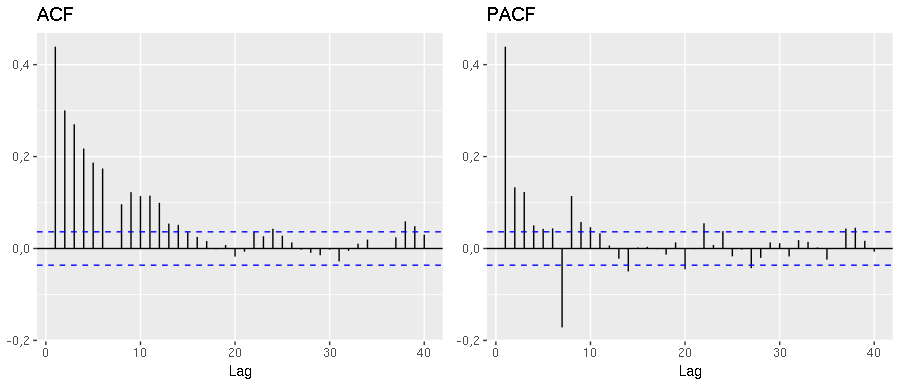
\includegraphics[width=\linewidth,height=5cm]{imgs/ACF_2.png}
  \caption{ACF e PACF dei residui del primo modello.}
  \label{fig:ACF_2}
\end{figure}
\begin{figure}[!h]
  \centering
  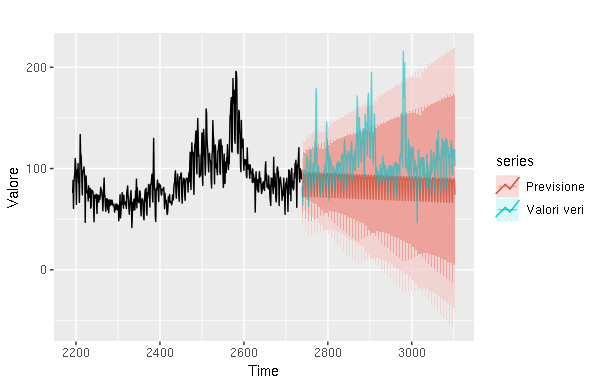
\includegraphics[width=\linewidth,height=6cm]{imgs/forecast_ar_1.png}
  \caption{Previsione della Serie sul Validation.}
  \label{fig:ARIMA_pred}
\end{figure}\\
Dalle previsioni di questo modello, mostrate nella Figura \ref{fig:ARIMA_pred}, si capisce immediatamente che queste componenti non spiegano tutta la varianza del modello, infatti questa serie è una serie multi stagionale, R non permette di trattare ARIMA multi stagionale quindi si introducono dei regressori esterni.\\
Per risolvere il problema di multi stagionalità si usano 24 regressori sinusoidali con frequenza base annua, il numero 24 è stato calcolato usando il validation set.
Si aggiungono altri regressori esterni: i giorni festivi, dando più importanza alle festività più importanti come il natale, pasqua, ferragosto e il nuovo anno e raggruppando le altre festività in un'unica variabile.
\begin{figure}[!h]
  \centering
  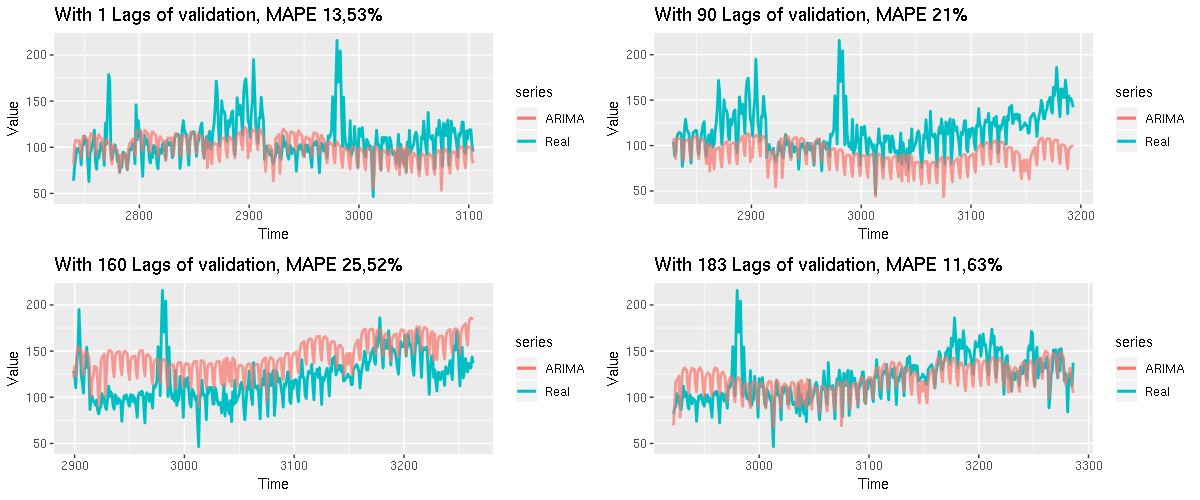
\includegraphics[width=\linewidth,height=6cm]{imgs/forecast_arima.png}
  \caption{Previsione su alcuni elementi del validation usando XARIMA.}
  \label{fig:XARIMA_pred}
\end{figure}\\
Nella figura \ref{fig:XARIMA_pred} si vede subito che questi regressori spiegano molta varianza del modello.\\
Il MAPE sul validation è $17.89\%$. 
%test di Dickey-Fuller
\section*{UCM}
Usando le considerazioni fatte per l'ARIMA si usa un modello UCM con un local linear trend, una componente stagionale settimanale stocastica con dummy e una componente stagionale stocastica annua con 24 regressori trigonometrici.
Si provano due modello: il primo usando i regressori per le vacanze costruite per l'ARIMA e il secondo senza l'ausilio di questi regressori.
per il validation si usa il predict di SSModel, che a sua volta sfrutta KFS, ma in questo modo è più facile introdurre nuovi dati nel modello senza rivalutare i suoi parametri.
Per il predict di SSModel bisogna passare il modello fittato usando i dati di train e un altro modello sempre della classe SSModel con gli stessi parametri ma con dati del validation seguiti da NA laddove bisogna fare predire al modello usando l'algoritmo di Kalman.\\
Sorprendentemente il modello senza regressori ottiene un MAPE più basso rispetto al modello con i regressori, quindi si opta per usare il modello UCM senza i regressori.\\
Il MAPE sul validation del modello con regressori è $19.21\%$ mentre del modello senza regressori è $18.06\%$. Nella Figura \ref{fig:UCM_pred} sono presente alcune stime effettuate sui dati del validation con i relativi errori.
\begin{figure}[!h]
  \centering
  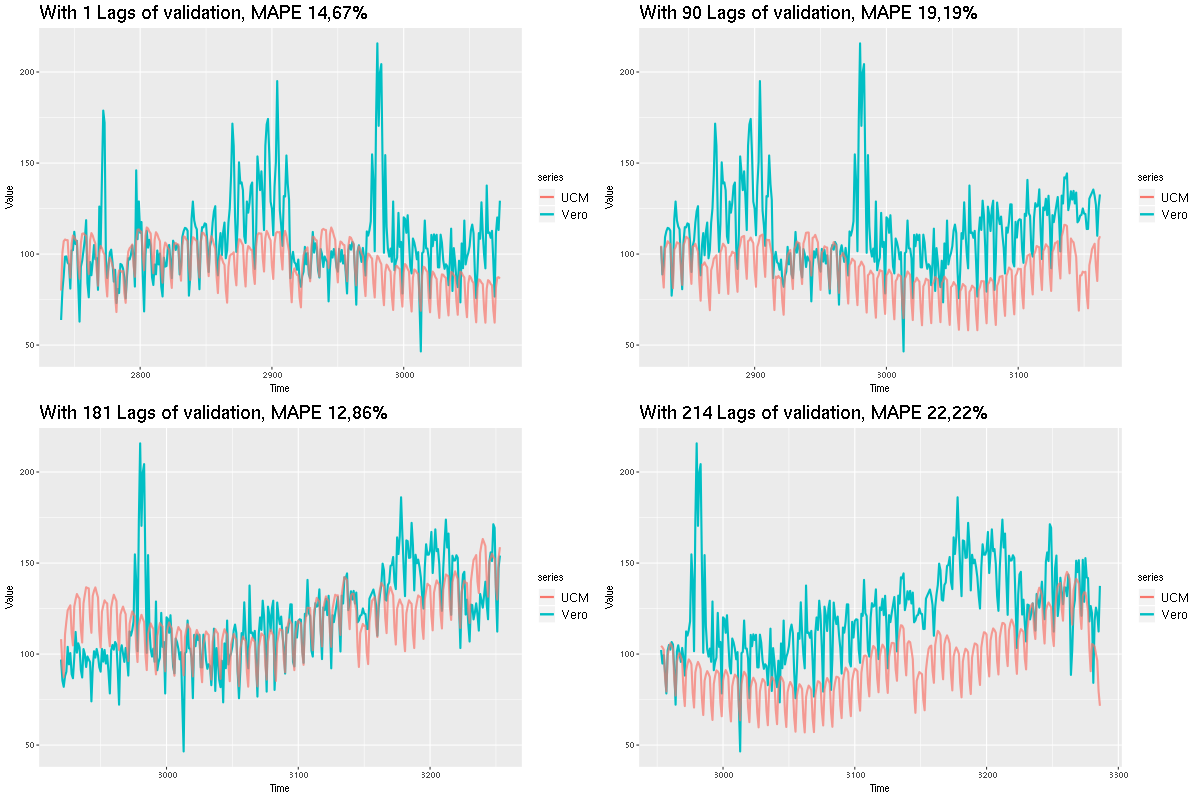
\includegraphics[width=\linewidth,height=6cm]{imgs/forecast_ucm.png}
  \caption{Previsione su alcuni elementi del validation usando UCM.}
  \label{fig:UCM_pred}
\end{figure}\\

\section*{LSTM}
Come ultimo modello è stato usato una rete neurale con nodi LSTM, sono stati testati anche le alternative come GRU o le più semplici RNN senza avere dei risultati migliori rispetto allo LSTM (in realtà le GRU avevano prestazioni molto simili alle LSTM).\\
Il train e validation è lo stesso usato per ARIMA e UCM in modo da renderli confrontabili.
I dati vengono standardizzati per avere media 0 e varianza 1, dove la standardizzazione si ottiene dal training set.
I dati vengono modificati per avere una struttura più adatta per il machine learning in generale, quindi si fissa L'INPUT\_SIZE che rappresenta quanti istanti temporali può guardare indietro il modello per prevedere n istanti successivi indicati con OUTPUT\_SIZE.
In questo caso OUTPUT\_SIZE è 365 visto che l'obiettivo è prevedere un anno di dati, mentre INPUT\_SIZE è 730 giorni che è un buon compromesso tra avere un numero di dati sufficiente per l'allenamento della rete neurale e un grado di informazione sufficiente per la previsione.\\
Sono state provate tre architetture:
\begin{itemize}[leftmargin=*]
\item Input$\to$LSTM(tanh)$\to$Dense(relu)$\to$Dense(relu)$\to$Output.
\item Input$\to$LSTM(tanh)$\to$Dense(relu)$\to$Dense(relu)$\to$Dense(relu)$\to$Output.
\item Input$\to$LSTM(tanh)$\to$LSTM(tanh)$\to$Dense(relu)$\to$Dense(relu)$\to$Output.
\end{itemize}
L'ottimizzatore di tutte e tre i modelli è RMSprop e la loss è `mse'. Gli iper-parametri di questo modello: il numero di unità LSTM, il numero di neuroni nei layer fully connected, il learning rate iniziale e il batch size, sono stati calcolati usando AutoML.
Inoltre nell'allenamento sono stati due callbacks di keras: uno per diminuire il learning rate in caso il modello non migliori sulla validation loss per almeno tre volte di seguito e uno per fermare l'allenamento nel caso il modello non migliori per oltre 50 epoche.
Il numero di epoche invece viene fissato a 100, che non è un numero ottimizzato ma compensato dall'esistenza dei callbacks.\\
Per AutoML è stato scelto come score la validation loss (mse) e come modello surrogato è stato scelto il GP con la EI come funzione di acquisizione, la libreria di python usata è sherpa-ai, che usa GPyOpt per l'ottimizzazione gaussiana, il numero di iterazioni è 100.\\
Nella Figura \ref{fig:automl} è indicato l'andamento dell'ottimizzazione utilizzando processi gaussiani per la prima architettura.
\begin{figure}[!h]
  \centering
  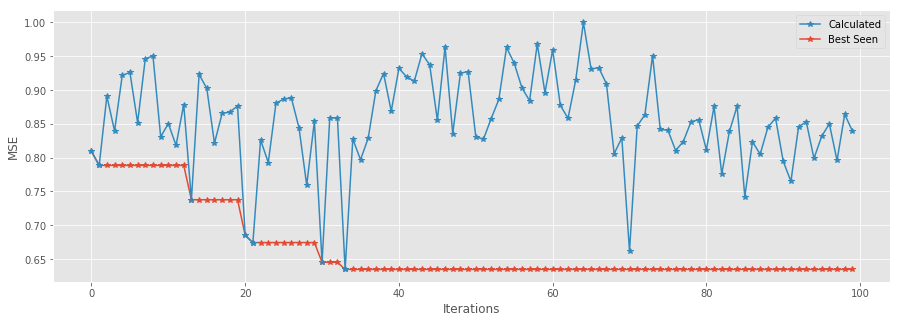
\includegraphics[width=\linewidth,height=4cm]{imgs/automl_1.png}
  \caption{Risultati del AutoML.}
  \label{fig:automl}
\end{figure}\\
Il miglior modello delle tre architettura dopo AutoML ottiene i seguenti MAPE sul validation:
\begin{enumerate}[noitemsep, topsep=0ex]
\item Primo: $14.53\%$
\item Secondo: $16.16\%$
\item Terzo: $16.25\%$
\end{enumerate}
Il miglior modello è il primo, nella Figura \ref{fig:LSTM_pred} vengono mostrate le sue previsioni per gli stessi validation del ARIMA e UCM.
\begin{figure}[!h]
  \centering
  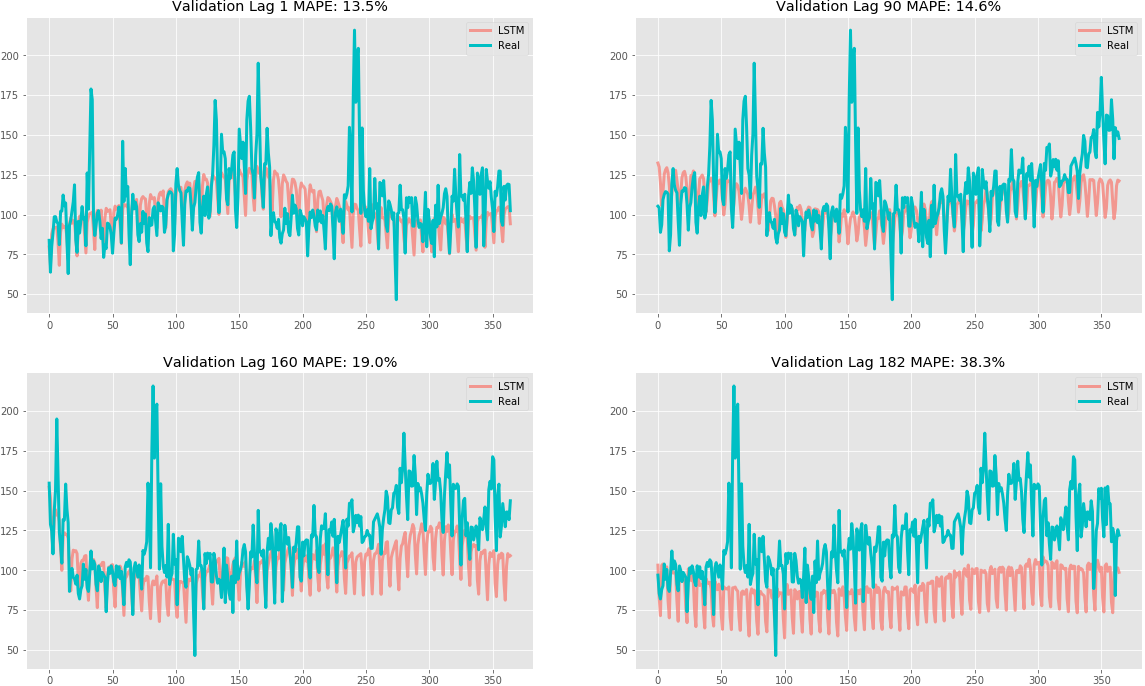
\includegraphics[width=\linewidth,height=6cm]{imgs/forecast_lstm.png}
  \caption{Previsione su alcuni elementi del validation usando LSTM.}
  \label{fig:LSTM_pred}
\end{figure}
%no way to use regressors in prediction easily
\section*{Conclusion}
I risultati delle tre metodologie sono:

\begin{table}[!h]
  \centering
  \begin{tabular}{|l|c|c|c|}
    \hline
    Model & ARIMA & UCM & LSTM\\
    \hline
    Training & $9.09\%$ & $10.98\%$ & $13.81\%$\\
    Validation & $17.89\%$ & $18.06\%$ & $14.53\%$\\
    \hline
  \end{tabular}
  \caption{Confronto dei risultati ottenuti dalle tre metodologie }
  \label{tab:confronto}
\end{table}
% reallenamento modello per previsione sul test


\end{document}